\documentclass[../_main/handlingar.tex]{subfiles}

\begin{document}
\beslutsuppfoljning{Representationsklädsel åt Inspektorn}
På Vårterminsmötet 2017 beslutades det att köpa in en mantel till Inspektorn.

Manteln köptes in och har överlämnats till Inspektorn som blev väldigt glad! Kostnaden uppgick till \SI{2280}{kr} vilket är under budgeten på \SI{2500}{kr}.

\begin{center}
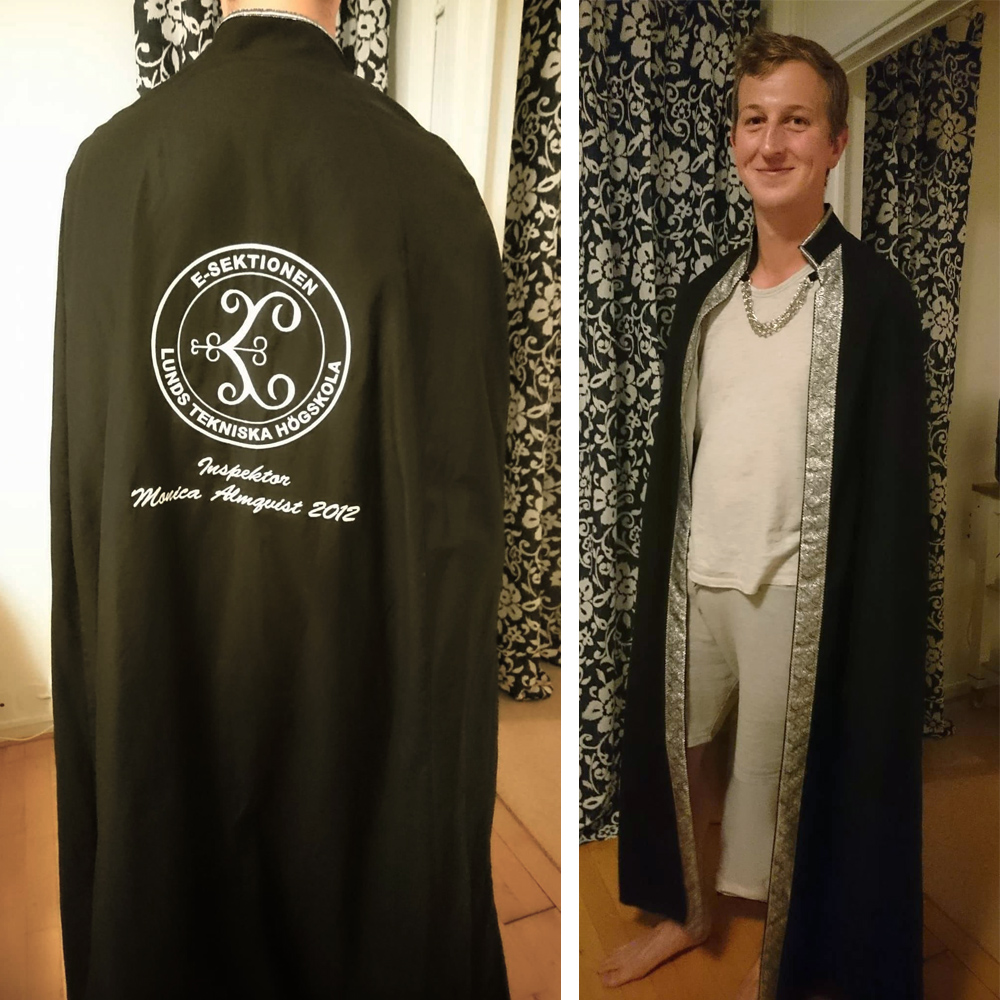
\includegraphics[scale=1.2]{mantel}
\end{center}

Med anledning av ovanstående yrkar styrelsen på

\begin{attsatser}
    \att stryka \emph{Representationsklädsel åt Inspektorn} från beslutsuppföljningen.
\end{attsatser}

\begin{signatures}{1}
    \ist
    \signature{\ordf}{Ordförande}
\end{signatures}

\end{document}
